% Report section types:  \part{}, \chapter{}, \section{}, \subsection{}, \subsubsection{}, \paragraph{}, \subparagraph{}.
% Article section types: \part{}, \section{}, \subsection{}, \subsubsection{}, \paragraph{}, \subparagraph{}.
\documentclass[a4paper]{article}

\marginparsep = 0pt
\marginparwidth = 0pt
\oddsidemargin = 0.5in
\textwidth = 5.25in
\usepackage{graphicx}
%\documentclass{report}
%\usepackage{fontspec}
\usepackage{hyperref}
%\setmainfont[Ligatures=TeX]{TeX Gyre Bonum}
%\setsansfont[Ligatures=TeX,Scale=MatchLowercase]{Latin Modern Sans}
%\setmonofont[Scale=MatchLowercase]{Inconsolata}
%\setmainfont[Numbers=Lining]{TeX Gyre Pagella}
\usepackage{lmodern}
\linespread{1.1}% spread lines out a little
\frenchspacing % remove extra space after punctuation
%:
\begin{document}
\title{\textbf{oscaar}: Open Source Differential Photometry Code for Amateur Astronomical Research}
\author{Brett Morris}
\maketitle
\tableofcontents
%\setcounter{tocdepth}{1}
\section{Introduction}

\newcommand{\oscaar}{$ \mathtt{oscaar}$ }
\newcommand{\code}[1]{\texttt{#1}}
\newcommand{\init}{\code{init.par}\ }

\oscaar's core is a differential photometry package built for users of any experience level at observatories of any size. The process of differential photometry can be applied to many astrophysical phenomena including transiting extrasolar planets, variable stars, rotating asteroids and more. This package is prepared specially for transiting exoplanet observations, though often other photometric observations can be analyzed with \oscaar without any tweaking to the source code.

Development for \oscaar began in the summer of 2011 to take a series of images obtained at the \href{http://www.astro.umd.edu/openhouse/}{University of Maryland Observatory} in College Park, MD, USA and churn out light curves of transiting extrasolar planets. If you're looking to do something similar, you've found the right code! The core of the code is written in \href{http://www.python.org/}{Python}, but it has been designed to be operated with a graphical user interface (GUI) for users who have never seen Python before. That being said, experienced programmers will find that the guts of \oscaar provide a well-documented toolkit for even the most demanding of photometric measurements. Since the v1.0 release, \oscaar has been used by astronomers at all levels, from undergraduates to observatory-directing IAU members.

Here we summarize the contents of this documentation. If you are new to photometry, you may consider reading Section \ref{sec:collectingData}, which will summarize observing techniques to make successful photometric measurements. In Section \ref{sec:run}, we will detail how to run \oscaar from the graphical user interface (GUI) or other ways without directly coding in Python. In Section *** we discuss the classes and methods that are built into \oscaar that users with programming experience may find useful to design their own analysis tools. 

\subsection{System Requirements} \label{sec:systemRequirements}

There are several packages in addition to Python that must be installed on your machine before running \oscaar. Most of these packages have been around for some time in the astronomical community. They are all free and available for download via links below. We apologize for the number of packages that are necessary to download, but we have decided that these packages enable for the most efficient open-source distro that we can provide.  \\ \\
\noindent
\indent \href{http://www.python.org/getit/}{\textbf{Python 2.7.X}}: The core language of oscaar \\
\indent \href{http://new.scipy.org/download.html}{\textbf{NumPy 1.6.0-py2.7}}: A Python module for efficient scientific computations \\
\indent \href{http://www.stsci.edu/resources/software_hardware/pyfits/}{\textbf{PyFITS 2.4.0}}: A Python module for handling FITS files \\
\indent \href{http://matplotlib.sourceforge.net/index.html}{\textbf{Matplotlib 1.X-py2.7}}: A Python module for plotting\\
\indent \href{http://www.wxpython.org/download.php#stable}{\textbf{wxPython}}: A Pythonic GUI toolkit \\
\indent \href{http://rhodesmill.org/pyephem/}{\textbf{PyEphem}} (\textit{optional}): A Python module for ephemeris generation \\

\noindent
PyEphem is not required to run differential photometric analysis with \oscaar but enables you to make detailed plans for observing nights in advance. More on this in Section ***.%\ref{}

\subsubsection{Disclaimer}

Though the modules used in this package have been stable historically and probably will not go away any time soon, the \oscaar Team does not take any immediate responsibility for problems that arise as a result of changes to future versions of these modules. 

\section{Collecting Data} \label{sec:collectingData}

\subsection{Picking A Target}



\subsection{Navigating The Sky} \label{sec:nav}

It is one hour before the photometric event that you want to observe, you have taken your flat fields, and you're ready to slew to your target. You punch in the RA and declination of the target, and your telescope lumbers over to that part of the sky, but you can't recognize the pattern of stars that come out on your first image. Is that star near the center of the field actually your target, or are you looking at the wrong part of the sky? 

While it is not necessary for running \oscaar, we highly recommend that you download the open-source planetarium software \href{http://www.stellarium.org/}{Stellarium} for navigating the sky and planning. This free, user-friendly package is supported on nearly every operating system and boasts some advanced features that will make it easy for you to find your targets. 

One feature of particular utility for the exoplanet community is that the object finding search bar that you use to find objects in Stellarium is linked to the professional astronomical database \href{http://simbad.harvard.edu/simbad/}{SIMBAD} to resolve nearly any object by any name. SIMBAD is updated relatively quickly, so when you want to go out and observe that new exoplanet but your old planetarium software doesn't know about the latest WASP or HAT target, Stellarium will resolve the name through SIMBAD and take you to the coordinates published for that object\footnote{Of course, this feature only works when your machine is connected to the internet, so if you do not have an internet connection at your observatory, you'll still need to query for your target before you get to the observatory, print out your star charts.}.

Stellarium also has great ``Flip Scene'' buttons that allow you to mirror flip your views of the sky to match the flips that your telescope optics do. That way you can match up your observed field of view with the stars in Stellarium without having to imagine complicated image transpositions in your head.

\subsection{Telescope Tracking}

Differential photometry is generally done on a series of images of the same patch of the sky over a long period of time. You'll need a telescope that is well polar-aligned so that the telescope's tracking keeps the stars in nearly the same spot on your detector throughout the duration of your observations. It is an unreasonable challenge to align most small telescopes well enough to track a star perfectly over several hours, so \oscaar is built to monitor and correct for the drift in star positions on the detector over time. Just make sure your target object and a few comparison stars stay in the field throughout the whole observation\footnote{If you need to re-center your target in the middle of an observation, \oscaar will only be able to continue to track the stars without special code tweaking if you change the stars' centroid positions by a few pixels (i.e., $\sim$2 or 3 pixels) at a time in between each exposure. The current version of \oscaar is not resilient against sudden discontinuous tracking anomalies.}. The star tracking algorithm follows each star individually over time. If your photometric target is an asteroid, for example, that moves relative to the comparison stars over time, \oscaar will happily track the asteroid and the comparison stars independently. 

\subsection{Defocusing} \label{sec:defocusing}

In precision photometry, relying on individual pixels is dangerous. Pixel defects occur frequently that can cause a pixel to read much higher counts than they actually receive (these are called ``hot pixels'') or sometimes much lower counts (``dead pixels''). If your target object is perfectly focused on a few pixels, you may be putting all of your photometric-eggs in one basket. Thus it is often advised that you \textbf{do not focus the telescope perfectly} when doing photometric measurements. If you can, defocus the telescope significantly so that you spread out the starlight over a few of pixels, and your pixel-to-pixel variations will play a less-significant role in the introduction of unwanted systematic noise and bias. See Figure \ref{fig:defocus} for examples.

Some photometry codes prefer objects focused in Gaussian-like shapes, but \oscaar is written to accurately track stars of unconventional shapes. At the University of Maryland Observatory, we make most of our measurements on a 6in refractor. We defocus the stars until they look like small donuts (the hole is an artifact of the optical path of the refractor), and we've found that our photometry comes out best this way. \oscaar won't complain if your stars are donut-shaped, Gaussian or somewhere in between. 

\begin{figure}[h]
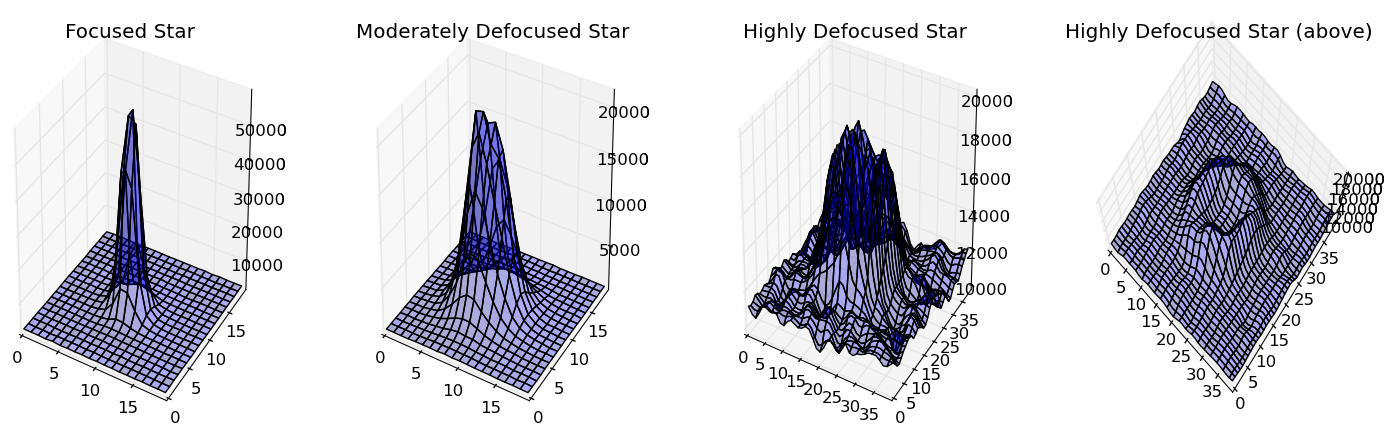
\includegraphics[scale=0.34]{imgs/focusing.png}
\caption{Images of stars with varying levels of defocusing. The $x$ and $y$ axes are the pixel indices, intensity in counts is plotted along the $z$. \oscaar can track any of these stars with precision -- even when the shape of the star is not approximately a Gaussian, like the highly defocused star on the right which is shaped like a donut.}
\label{fig:defocus}
\end{figure}

One must keep in mind that by spreading out the light over many pixels, the counts measured by each pixel is lower. As a result, defocusing is most helpful when observing bright objects. If the source you are observing is bright enough, you can defocus significantly without losing too much signal. However, it is important to note that the quality of your light curve will be directly related to how much more signal than noise you detected, as we will discuss in Section \ref{sec:photonNoise}. Use defocusing sparingly (or not at all) when imaging dim targets\footnote{For example, we use a sharp focus for stars dimmer than $V=10$ on our 152mm refractor at the University of Maryland Observatory.}.

\subsection{Theory: Photon Noise} \label{sec:photonNoise}

There is a fundamental physical limit to the signal-to-noise ratio that can be achieved in photometric measurements. Since photometry is the process of counting photons, there is a type of statistical uncertainty introduced into each measurement that goes by many names: \textit{photon noise, Poisson uncertainty, shot noise,} etc. This uncertainty is unavoidable in counting measurements and is easy to calculate -- the photon noise, or the uncertainty in a measurement of $N$ photons, $\sigma_N$ is

\begin{eqnarray}
\sigma_N = \sqrt{N}. \label{eqn:photonNoise}
\end{eqnarray}

\noindent You can see directly from Equation \ref{eqn:photonNoise} that the fractional uncertainty in the signal ($\sigma_N/N$) decreases with increasing $N$ as $1/\sqrt{N},$
so the more signal you have, the lower the limiting fundamental uncertainty. Of course, in practice there are many additional noise sources that will add uncertainty into your data and increase the scatter in your light curves. 
 
\subsection{Dark Fields and Flat Frames}

Collecting dark frames and flat fields is standard practice for removing systematic effects from CCD images. Flat fields correct for dust and other inconsistencies in the optical path artificially brighten or dim the objects that you image. Dark frames remove some flaws in the CCD like hot pixels and dark current variations. Some CCD imaging software like MaxIm DL have easy preset routines for taking dark frames.  We recommend taking $\ge8$ dark frames for each set of observations you take. \oscaar will take the mean of these sets and apply them appropriately to each image of your data set. 

Collecting good flat fields can sometimes be more of an art than a science, but good flats are important for good photometry. For this reason, we've incorporated two methods of ``master flat'' making routines into \oscaar, that combine raw flat fields into one master flat. The first method is called the ``Standard'' method by the \oscaar GUI, which takes a mean of all of the input flat frames. This is the fastest computational method. Standard master flats are ideal for ``dome flats'', where the flat fields are obtained by imaging a screen. Many astronomers prefer ``twilight'' or ``sky'' flats, in which the telescope takes images of the sky as the sun sets, and light from the sky acts as the uniform light source. We developed a corresponding twilight master flat setting for \oscaar, which fits a linear function to the intensity of each pixel over time, and uses the best-fit intercept as the normalizing factor for the master flat. Since loops are slow in Python, this method may take a few minutes to produce a master flat, but the payoff that you gain in photometric precision is worth the wait. At the time of writing, we're currently investigating how to implement these algorithms in \href{http://www.cython.org/}{Cython} to help us speed up these expensive computations.

\subsection{Picking A Target}
\subsubsection{Transit Predictions}
So you're planning a night of transiting extrasolar planet observations, and you need to know what planets are transiting during your local night. We recommend using the \href{http://var2.astro.cz/ETD/predictions.php}{Czech Astronomical Society Exoplanet Transit Database's Transit Prediction tool}. If you enter your latitude and longitude, this web-tool will tell you which bright transiting extrasolar planets will be visible and transit on a given night from your location. This tool is invaluable for planning. It's also great because you can contribute to this database by submitting your light curves to help constrain the orbital parameters of the planets. With a telescope and \oscaar, you can contribute to real science!

\subsubsection{Choosing The Field}
When you chose your target for differential photometry, you need to be sure there are other stars in the imaging field. Here we'll define some terms that are important from here on:  \\ 

\noindent \textbf{Target Star}: The target of your observations -- the host star to an exoplanet or the variable star that you're measuring for intrinsic variations in luminosity. Of course, this ``star'' could be an asteroid, if you're into that sort of thing. \\\\
\textbf{Comparison Star}: A star other than the target star that you will use as a basis for determining the intrinsic variations in the brightness of the target star. The comparison star should be one that is not known to have intrinsic variations. \\

There must be at least one comparison star in order to do differential photometry, and the more the better. There is no magic number of comparison stars to have, but if you have the opportunity to fit more control stars in the field by rotating your CCD or effectively ``zooming out," it will be worth your while. Based on prior experience with \oscaar, more than two good stars will suffice, but 10 can give you great results. Later, we'll discuss how to know which ones are ``good.''

Photometry of bright stars is always preferable to dim stars, but of course there are more dim stars than bright stars in most of the images you will take. In order to avoid uncertainty introduced noise with very dim stars, pick control stars with peak intensities more than double the average background intensity in the area surrounding the star. 

Different transiting exoplanets change the brightnesses of their host stars by different amounts. This parameter is called ``\textbf{depth}" and is often measured in units of millimagnitudes (mmag). The greater the depth of a transit, the more likely you will be capable to detect the transit. Since some of these depths are so small, it might is a good idea to perfect measuring \href{https://sites.google.com/site/aavsosppsection/}{short period pulsating (SPP) variable stars} with high amplitude luminosity oscillations (like \href{http://www.aavso.org/vsx/index.php?view=detail.top&oid=4356}{YZ Boo}) before you move on to exoplanets. Once you characterize your ability to measure the large intrinsic variations of variable stars, you will be able to characterize your ability to detect the small depth regime of transiting exoplanets. 

\subsection{Imaging Software}
A bunch of imaging packages could suite your needs for photometry with \oscaar. At the University of Maryland Observatory, we use \href{http://www.cyanogen.com/maxim_main.php}{MaxIm DL} to handle our imaging. Any imaging software that enables you to take a time-series of CCD images will do. 

Observing software like MaxIm DL allow you to choose your imaging \textbf{binning}, which enables the detector to read-out pixels in groups. For example, a $2\times2$ binning will take a square of four pixels and save them as one composite pixel. This reduces the read-out time, the size of the output files, and the run time of scripts that have to read and manipulate those images. We recommend that you use $2\times2$ binning when you can for these reasons. It is often unimportant to save images at the full-resolution of the detector, especially when you are using defocusing anyway, as described in Section \ref{sec:defocusing}. 

\section{Running \oscaar v2.0}

The first step in running ocaar 2.0 is to execute the oscaarGui.py python file which is located in the OSCAAR folder that you downloaded. This should bring you to a screen that looks something like this:

****Insert Screencap here****

You will now be shown some initial parameters that you must set in order to run \oscaar.

%\subsection{Pickling your FITS files}

\subsection{Locating Your Stars with DS9}

The first and most intensive task you'll have to do to prepare \oscaar  for analysis is to tell it what stars you care about in your images. If you have a set of images, there could be tens or hundreds of stars in each image, some of them close to the edges, some of them with binary companions; some of them ideal control stars, some of them not. In order to ensure that the stars being picked as control stars are appropriate choices, \oscaar has the user enter each of the stars into \oscaar with the help of SAO Image DS9 (see Section \ref{sec:systemRequirements} to download). 

To begin, start DS9 and open the first image from the series of images you will process. You can also start DS9 from within \oscaar by clicking \code{Open DS9} button. Set the scale and zoom so that you can see most of the image and most of the stars in it. With the mouse set to \code{Pointer} (\code{Edit} \textgreater  \code{Pointer}), click on the target star (the exoplanet host star or variable star). A green circle will appear over the star along with a dialogue box which contains the pixel coordinates of the circle's center and radius, see Figure \ref{fig:ds9}. 
\begin{figure}[h]
\begin{center}
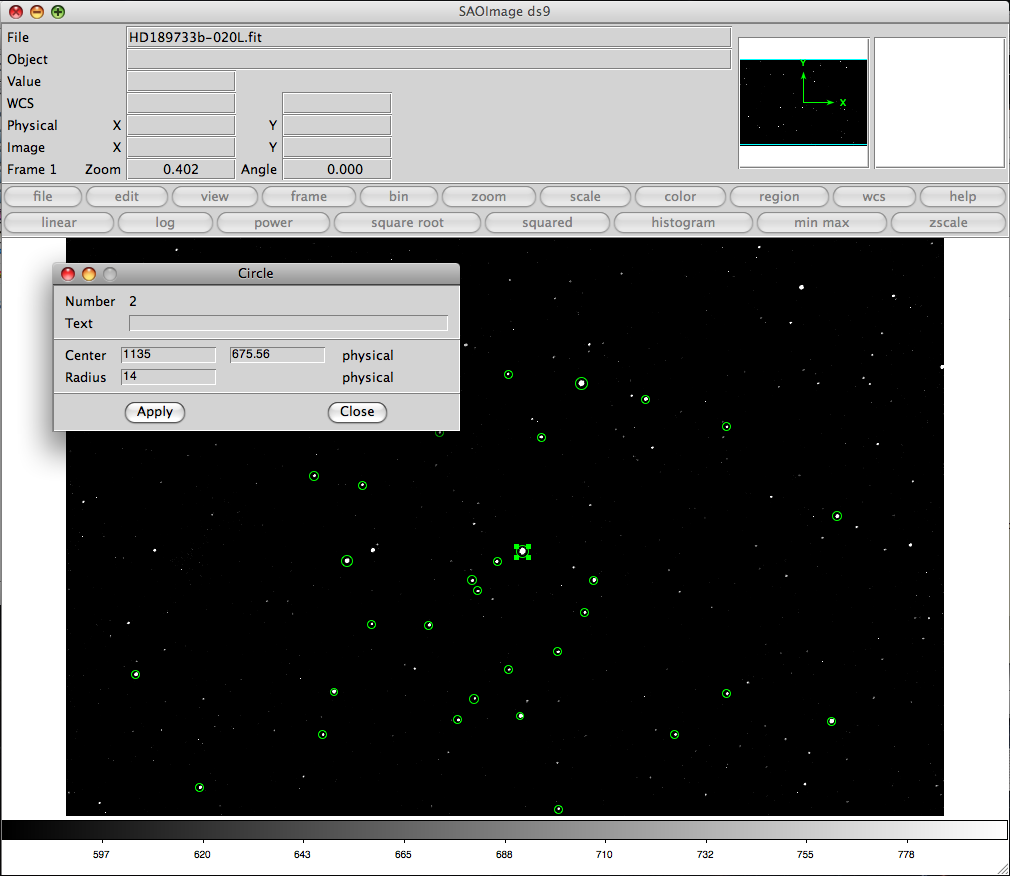
\includegraphics[scale=0.2]{imgs/ds9.png}
\caption{Using DS9 to locate the target and comparison stars.}
\label{fig:ds9}
\end{center}	
\end{figure}
The first star that you select will be treated as the target star, and any subsequent choices will be comparison stars. Repeat this process for as many comparison stars as you like (try to keep it under 25 for speed). Avoid picking stars near any obvious defects on the detector, any stars less than 150 pixels from the edge of the image, or stars with a neighboring star close nearby. 

When you're done choosing control stars, go to \code{Regions} \textgreater  \code{Save Regions...} and save a regions file in a directory where you will be able to find it later. This file will contain the pixel coordinates of the stars at the beginning of the observation, which tells \oscaar which stars to track. You may want to check that the test star is in fact the first star in the regions file. Open the regions file in a text editor and check that the first line resembling ``\code{circle(100,600,10)}'' has the proper (x,y) pixel coordinates and radius (in this example, the position is (100,600) with a radius of 10). If the first circle coordinate line does not point to the target star, find the circle coordinate that does, move that line to the top of the list, and save the file.

In the \oscaar GUI, click \code{Browse} in the \code{Path to Regions File} field and enter the path to the regions file you just made.

\subsubsection{Locating Your Data}

	\oscaar  is built to find files by their paths. To properly set the image paths, you should click the browse button next to the dark images path field and choose all of the dark image files that you wish to be processed. To do this, select your first file, then hold the \code{Ctrl} key on Windows or the \code{Command} key on Mac and click every file you would like to select. Alternatively, if they are all listed consecutively, you can click the first file, hold shift, and then click the last one. Now click the ``Open'' button and all of your dark images should be listed separated by commas. Do the same for your data images in the \code{Data Images} field of the \oscaar GUI.
	
\subsection{Making a Master Flat}
Now that you have properly set the path to the darks and the data images, you must now make your master flat. First click the ``Master Flat Maker'' button at the bottom of the \oscaar window, and a dialog box should pop up that looks like Figure \ref{fig:flats}.
\begin{figure}[h]
\begin{center}
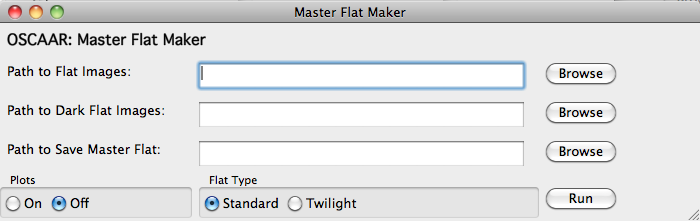
\includegraphics[scale=0.25]{imgs/flatMaker.png}
\caption{\oscaar's Master flat maker allows you to make master flats out of raw images.}
\label{fig:flats}
\end{center}	
\end{figure}

Now you must set the paths to the flat images and the dark flat images in the same way you set the image paths previously. You must also enter the path and filename for the master flat. To do this, click the \code{Browse} button and navigate to the location you would like to save the master flat. 

There are two options for how you can make your flat, either  the ``Standard'' or ``Twilight'' flat type. The standard flat maker algorithm is a simple mean combination of the flat frames that you enter into the flat maker GUI. If you took dome flats or bright sky flats, this is the right option for you. If you took flats at twilight as the sun was setting and the sky background was your ``screen'', the twilight flat algorithm will fit a linear function to the intensity of each pixel over time, and use the intercept as the normalization factor for the flat. The twilight flat algorithm is much slower than the standard method, because those linear fits are computationally expensive in an interpreted language like Python. We hope to code up alternative versions of these routines that you can experiment with on your dataset, some of which may access much faster, compiled code in C or Cython.

Now click the \code{Run} button on the master flat maker and close it when it is done. You should now choose the output file when selecting the path to the master flat frame in the main \oscaar GUI. 


\subsection{Running Parameters}
The next step in running \oscaar is to properly set all of the initial running parameters. These have default values set, but these may need to be modified for your particular data set.

\subsubsection{Smoothing Constant}


\begin{figure}[h]
\begin{center}
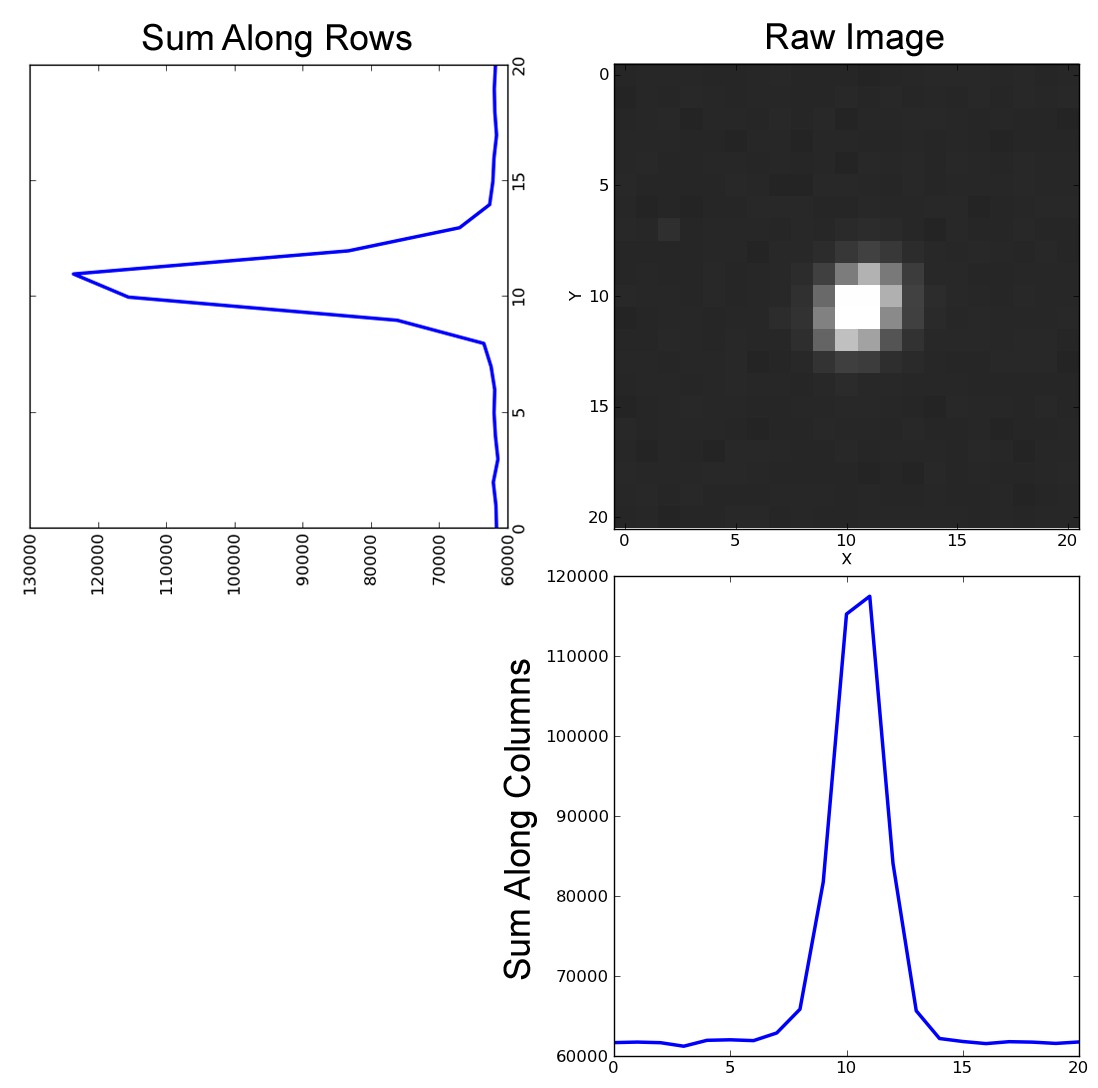
\includegraphics[scale=0.20]{imgs/sums.png}
\caption{Sums along the columns and rows around a star.}
\label{fig:sumsExample}
\end{center}	
\end{figure}

\begin{figure}[h]
\begin{center}
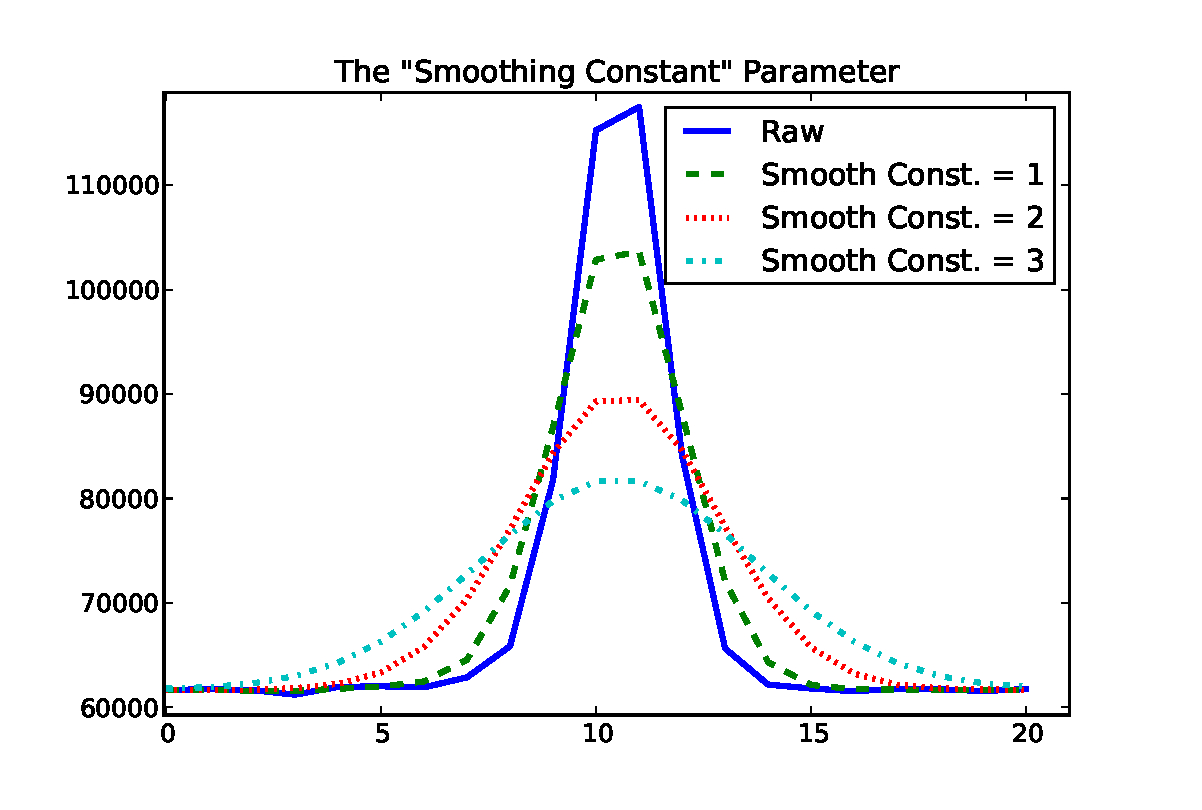
\includegraphics[scale=0.45]{imgs/smooth.eps}
\caption{A range of \code{Smoothing Constant} values from 0 to 3 are applied to the stellar intensity profile along the columns surrounding one star (see Figure \ref{fig:sumsExample} for the origin of the intensity profile).}
\label{fig:smoothExample}
\end{center}	
\end{figure}

\subsubsection{Tracking and Photometry Plots}

\begin{figure}[h]
\begin{center}
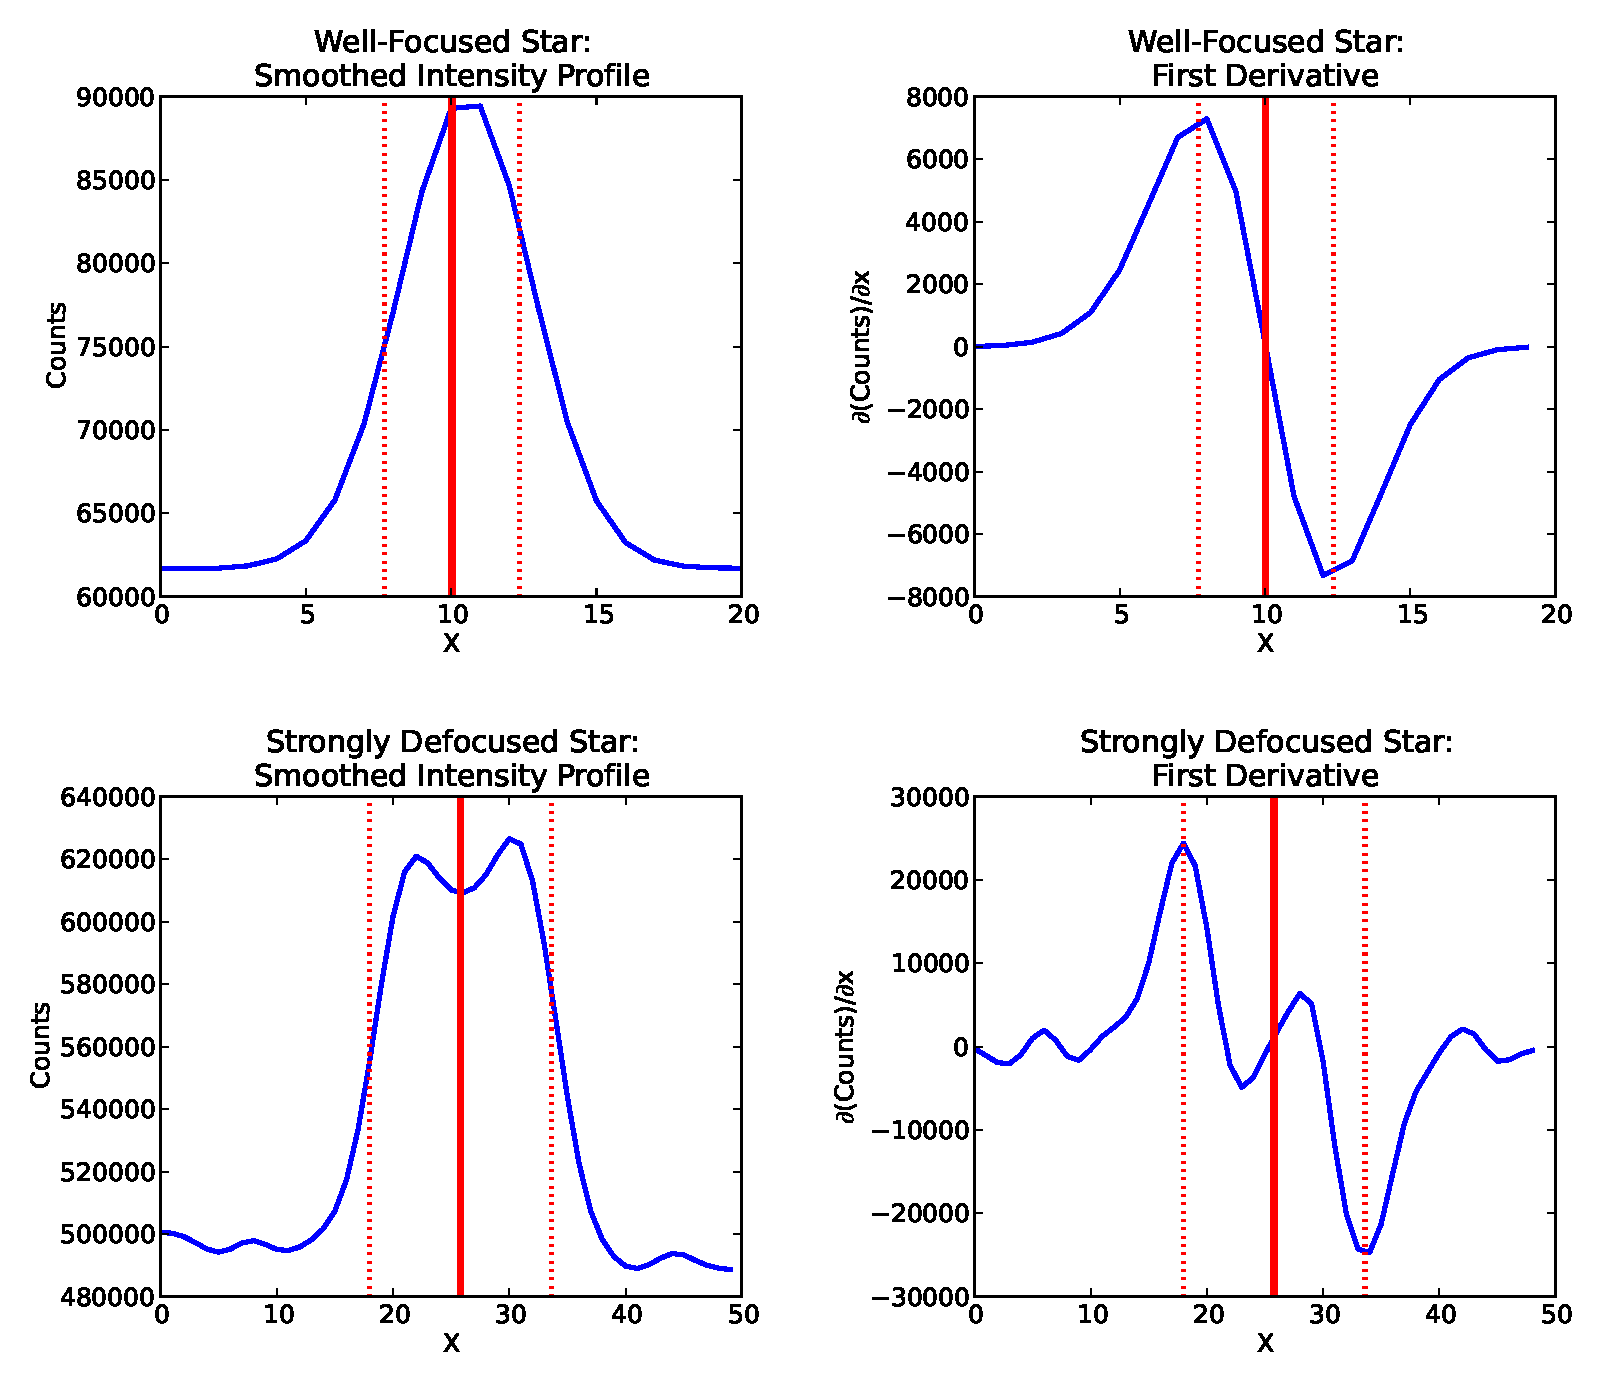
\includegraphics[scale=0.45]{imgs/trackingExample.eps}
\caption{\textbf{Stellar Centroid Tracking}: The top row of plots show the sum of intensities in each pixel along the columns a well-focus star, similar to Figure \ref{fig:sumsExample}, and the bottom row shows the same for a highly defocused star (see discussion on defocusing in Section \ref{sec:defocusing}). The plots on the left show the counts on the detector summed along the columns of pixels, and smoothed with non-zero smoothing constants. The plots on the right show the first spatial derivative of the intensity profiles, with clear extrema at the pixel locations corresponding to the points of greatest positive and negative slope in the intensity profiles. A quadratic is fit to the three points closest to each of the extrema, yielding sub-pixel precision measurements on the coordinates of the extrema (marked above with the dotted vertical red lines). The midpoint between these best-fit extrema is taken as the stellar centroid, marked with the solid vertical red line in the plots above. This process is repeated for the other axis (sum along the rows) to get the other of the two centroid coordinates for each star.}
\label{fig:sumRowsAndCols}
\end{center}	
\end{figure}



\begin{figure}[h]
\begin{center}
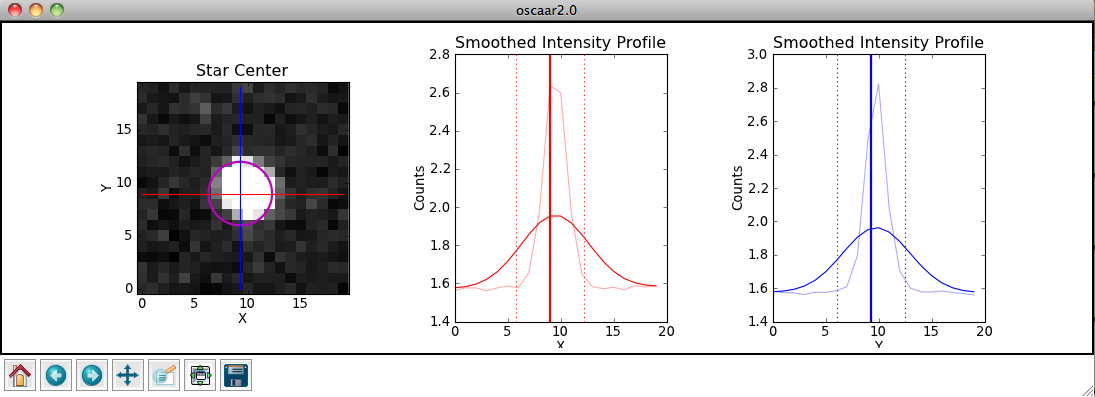
\includegraphics[scale=0.25]{imgs/trackPlots.png}
\caption{\code{Track plots} set to \code{True} and \code{Photometry plots} set to \code{False}. The leftmost image shows the star with a cross-hair indicating the centroid, also circled in magenta (the radius of this circle is not meaningful). The plots on the right indicate the sums of the intensities in pixels along the rows and columns, in the transparent curves. The solid curves represent the smoothed intensity profiles, which are used to find the centroid. The bold vertical lines mark the best-fit stellar centroid in each axis.}
\label{fig:trackingExamples}
\end{center}	
\end{figure}

\begin{figure}[h]
\begin{center}
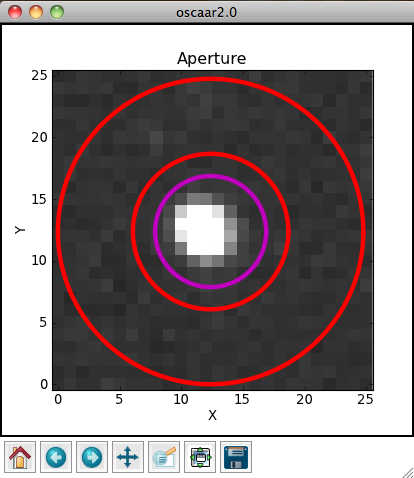
\includegraphics[scale=0.25]{imgs/aperPlots.png}
\caption{\code{Photometry plots} set \code{True} and \code{Track plots} set to \code{False}. The innermost circle (magenta) marks the \code{Aperture Radius} (see Section \ref{sec:aperRad}) measured from the stellar centroid found for this star by the tracking algorithm. All pixels that fall inside of this radius are summed to calculate the flux from this star. The next two concentric circles (red) mark the ``sky annulus,'' within which the sky background is measured.  }
\label{fig:photPlots}
\end{center}	
\end{figure}

\begin{figure}[h]
\begin{center}
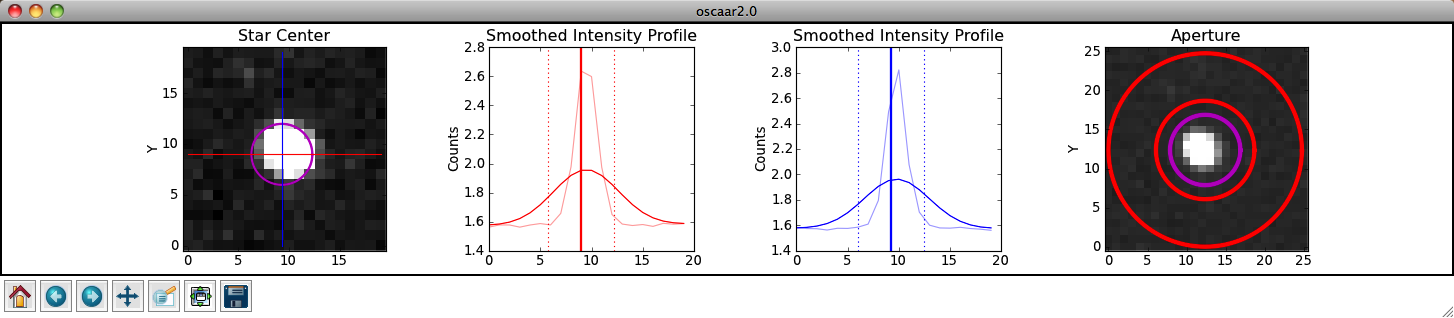
\includegraphics[scale=0.25]{imgs/trackAperPlots.png}
\caption{\code{Track plots} and \code{Photometry plots} both set \code{True}. See Figures \ref{fig:trackingExamples} and \ref{fig:photPlots} for more details on each subplot.}
\label{fig:trackAndPhotPlots}
\end{center}	
\end{figure}



\subsubsection{Track Zoom}
\oscaar tracks each star through consecutive exposures by looking for the each centroid near to the detector location that it had in the previous exposure. Since the stars will drift somewhat from frame to frame if your telescope is not perfectly aligned, we define a width around the previous centroid within which to search for the centroid in the following frame. The ideal width of this search box will depend on the plate scale of your device, how defocused the telescope is, how poor the alignment is, etc. 



\subsubsection{CCD Gain}


\subsubsection{Aperture Radius} \label{sec:aperRad}


\subsubsection{Notes}
This text field is meant for you to enter any notes you might want to know later. All of your running parameters will be saved in the data file so you won't need to copy them here, but if you want to label the run in any particular way, there's a sweet little box here specifically for that purpose.

\subsubsection{Ingress and Egress Times}
If you are observing a transiting exoplanet, \oscaar can do its most precise photometry if it knows when your target is ``in-transit'', meaning the planet is occulting the disk of star, or ``out-of-transit'', meaning the planet is not occulting the star. This is because it uses mathematical techniques that look for changes in each comparison star compared to the target star in order to determine which comparison stars are the best to use. If you compared the target to comparisons while the planet was in-transit, there would be a real (and important) difference between the two that we want to measure accurately. For this reason we input the ingress and egress times and only compare the target and comparison stars during out-of-transit exposures.

Enter the times in MM/DD/YYYY;  hh:mm format, where the hours are on the 24-hour scale, in Universal Time. Seconds are insignificant.



\section{Contributing to \oscaar}
This version of \oscaar was made by four people, and we're proud of the work we've done. But \oscaar can still be improved and we need your help! \oscaar is used in more than 10 countries by amateurs and professionals alike, and in order to keep up with the demands of providing a user-friendly differential photometry code for an international audience, we'd love to have your help if you can: code in Python, or provide any feedback at all. If you'd like to help but don't know where to begin, please feel free to contact us at \href{mailto:oscaarUMD@gmail.com}{oscaarUMD@gmail.com}. We'd love to work together! 

We keep the \href{https://github.com/OSCAAR/OSCAAR}{source code on GitHub}, a popular open source code repository site. There you can find the code in its most up-to-date (alpha, beta, and stable) form, the \href{https://github.com/OSCAAR/OSCAAR/issues?state=open}{Issue Tracker} where known issues are logged and new issues or comments can be posted.




\section{Acknowledgements}
\oscaar has come a long way from the first 1,000 lines of code that Brett Morris wrote in 2011. It could not have gotten there without the help of the following colleagues: 
Drake Deming, Avi Mandell, Daniel Galdi, Sam Gross, Luuk Visser, Harley Katz, Elizabeth Warner, Alberto Bolatto.

	
\end{document}